% slides.tex

\documentclass{beamer}
\usetheme{default}

\title{Data Structures for Range-Sum Queries}
\subtitle{The Evolution of the Data Cube}
\author{Paul Butler}
\institute{
    CUMC 2010\\
    Waterloo, Ontario
}
\date{July 2010}

\usepackage{amsthm}
\usepackage{tabularx,colortbl}
\usepackage{multirow}
\usepackage{cite}
\usepackage{subfigure}

\theoremstyle{definition}
\newtheorem{myexample}{Example}
\theoremstyle{definition}
\newtheorem{mynote}{Note}

\newcommand{\graycell}{\cellcolor[gray]{0.8}}

\begin{document}

\begin{frame}[plain]
    \titlepage
\end{frame}

\begin{frame}{The Range-Sum Problem: Example}
    \begin{table}[h]\footnotesize
        \begin{tabular}{ | l | l | l | l | l | l |}
        \hline
        \rowcolor{red!20!green!20!blue!20}
        \textbf{Name} & \textbf{Born} & \textbf{City} & \textbf{Height} & \textbf{Siblings} & \textbf{Pets} \\ \hline
        Joseph Matthews & Jan 9, 1987 & Waterloo & 172 & 2 &  1 \\ \hline
        Sarah MacDonald & Nov 17, 1988 & Halifax & 167 & 0 & 2 \\ \hline
        \vdots & \vdots & \vdots & \vdots & \vdots & \vdots \\ \hline
        \end{tabular}
    \end{table}

    \begin{itemize}
        \item<+-> How many people in Vancouver were born before 1990?
        \item<+-> What is the average number of siblings for people above 170~cm?
        \item<+-> What is the total number of pets owned by people 18 to 24 in Calgary?
    \end{itemize}
\end{frame}

\begin{frame}{The Range-Sum Problem: Definitions}
    \begin{definition}[Measure]
        A column whose values we want to aggregate in our queries.
    \end{definition}
    \pause
    \begin{myexample}
        The \textbf{Pets} and \textbf{Siblings} columns from the last example are \textbf{measures}
    \end{myexample}
    \pause
    \begin{definition}[Dimension]
        A column we want to use to select columns which belong to our aggregation.
    \end{definition}
    \pause
    \begin{myexample}
        The \textbf{Born}, \textbf{City}, and \textbf{Height} columns are \textbf{dimensions}.
    \end{myexample}
\end{frame}

\begin{frame}{Dimensions vs. Measures}
    \begin{itemize}
        \item<+-> For each column, \textbf{dimension} vs. \textbf{measure} depends on which questions you want to answer.
        \item<+-> \textit{What is the average age of people with two pets}
        \pause
        \begin{itemize}
            \item \textbf{Born} would be a \textbf{measure}
            \item \textbf{Pets} would be a \textbf{dimension}
        \end{itemize}
    \end{itemize}
\end{frame}

\begin{frame}{The Na\"{i}ve Approach}
    \begin{itemize}
        \item Store the data as a table
        \item For every row:
        \begin{itemize}
            \item If the dimension columns match our query, add the value in the measure column to a running total
        \end{itemize}
        \item Return the running total
    \end{itemize}
    \pause
    \textbf{Too slow} for large amounts of data!
\end{frame}

\begin{frame}{Data Cubes}
    We can aggregate the data into a multi-dimensional array.\cite{Gray96}

    \begin{table}[h]\footnotesize
        \begin{tabular} { | l | l | l | l | l | l | l | l | l |}
        \hline
        \textbf{Pets} & & \multicolumn{7}{|c|}{Born} \\ \hline
        & & $\hdots$ & 1985 & 1986 & 1987 & 1988 & 1989 & $\hdots$ \\ \hline
        \multirow{6}{*}{Height}
        & \vdots & $\ddots$ & \vdots & \vdots & \vdots & \vdots & \vdots & $\ddots$ \\
        & 165 & $\hdots$ & 192 & 342 & 558 & 56 & 591 & $\hdots$ \\
        & 166 & $\hdots$ & 325 & 275 & 707 & 855 & 484 & $\hdots$ \\
        & 167 & $\hdots$ & 487 & 326 & 363 & 193 & 350 & $\hdots$ \\
        & 168 & $\hdots$ & 326 & 363 & 193 & 350 & 422 & $\hdots$ \\
        & 169 & $\hdots$ & 438 & 456 & 550 & 385 & 412 & $\hdots$ \\
        & \vdots & $\ddots$ & \vdots & \vdots & \vdots & \vdots & \vdots & $\ddots$ \\
        \hline
        \end{tabular}
    \end{table}
    \pause
    Now cells not selected by the query are ignored. \\
    Less lookups, faster queries (but still too slow).
\end{frame}

\begin{frame}{Data Cubes}
    \begin{myexample}
        What is the total number of pets owned by people born between 1986 and 1988 and height between 166 and 168~cm?
    \end{myexample}

    \begin{table}[h]\footnotesize
        \begin{tabular} { | l | l | l | l | l | l | l | l | l |}
        \hline
        \textbf{Pets} & & \multicolumn{7}{|c|}{Born} \\ \hline
        & & $\hdots$ & 1985 & 1986 & 1987 & 1988 & 1989 & $\hdots$ \\ \hline
        \multirow{6}{*}{Height}
        & \vdots & $\ddots$ & \vdots & \vdots & \vdots & \vdots & \vdots & $\ddots$ \\
        & 165 & $\hdots$ & 192 & 342 & 558 & 56 & 591 & $\hdots$ \\
        & 166 & $\hdots$ & 325 & \graycell 275 & \graycell 707 & \graycell 855 & 484 & $\hdots$ \\
        & 167 & $\hdots$ & 487 & \graycell 326 & \graycell 363 & \graycell 193 & 350 & $\hdots$ \\
        & 168 & $\hdots$ & 326 & \graycell 363 & \graycell 193 & \graycell 350 & 422 & $\hdots$ \\
        & 169 & $\hdots$ & 438 & 456 & 550 & 385 & 412 & $\hdots$ \\
        & \vdots & $\ddots$ & \vdots & \vdots & \vdots & \vdots & \vdots & $\ddots$ \\
        \hline
        \end{tabular}
    \end{table}
    \pause
    275 + 707 + 855 + 326 + 363 + 193 + 363 + 193 + 350 = \textbf{3625}
\end{frame}

\begin{frame}{Data Cubes}
    We can calculate partial sums for each row, column, etc.\cite{Gray96}
    \begin{table}[h]\footnotesize
        \begin{tabular} { | l | l | l | l | l | l | l | l | l | l |}
        \hline
        \textbf{Pets} & & \multicolumn{8}{|c|}{Born} \\ \hline
        & & $\hdots$ & 1985 & 1986 & 1987 & 1988 & 1989 & $\hdots$ & Sum \\ \hline
        \multirow{7}{*}{Height}
        & \vdots & $\ddots$ & \vdots & \vdots & \vdots & \vdots & \vdots & $\ddots$ & \vdots \\
        & 165 & $\hdots$ & 192 & 342 & 558 & 56 & 591 & $\hdots$ & 10937 \\
        & 166 & $\hdots$ & 325 & 275 & 707 & 855 & 484 & $\hdots$ & 10998 \\
        & 167 & $\hdots$ & 487 & 326 & 363 & 193 & 350 & $\hdots$ & 11064 \\
        & 168 & $\hdots$ & 326 & 363 & 193 & 350 & 422 & $\hdots$ & 10913 \\
        & 169 & $\hdots$ & 438 & 456 & 550 & 385 & 412 & $\hdots$ & 11347 \\
        & \vdots & $\ddots$ & \vdots & \vdots & \vdots & \vdots & \vdots & $\ddots$ & \vdots \\
        & Sum & $\hdots$ & 8121 & 8255 & 8206 & 8820 & 8026 & $\hdots$ & 202169 \\
        \hline
        \end{tabular}
    \end{table}
    \pause
    Queries which only mention a subset of the dimensions now run faster.
\end{frame}

\begin{frame}{Data Cubes}
    \begin{myexample}
        How many pets are owned by people born between 1986 and 1988 (inclusive)?
    \end{myexample}

    \begin{table}[h]\footnotesize
        \begin{tabular} { | l | l | l | l | l | l | l | l | l | l |}
        \hline
        \textbf{Pets} & & \multicolumn{8}{|c|}{Born} \\ \hline
        & & $\hdots$ & 1985 & 1986 & 1987 & 1988 & 1989 & $\hdots$ & Sum \\ \hline
        \multirow{7}{*}{Height}
        & \vdots & $\ddots$ & \vdots & \vdots & \vdots & \vdots & \vdots & $\ddots$ & \vdots \\
        & 165 & $\hdots$ & 192 & 342 & 558 & 56 & 591 & $\hdots$ & 10937 \\
        & 166 & $\hdots$ & 325 & 275 & 707 & 855 & 484 & $\hdots$ & 10998 \\
        & 167 & $\hdots$ & 487 & 326 & 363 & 193 & 350 & $\hdots$ & 11064 \\
        & 168 & $\hdots$ & 326 & 363 & 193 & 350 & 422 & $\hdots$ & 10913 \\
        & 169 & $\hdots$ & 438 & 456 & 550 & 385 & 412 & $\hdots$ & 11347 \\
        & \vdots & $\ddots$ & \vdots & \vdots & \vdots & \vdots & \vdots & $\ddots$ & \vdots \\
        & Sum & $\hdots$ & 8121 & \graycell 8255 & \graycell 8206  & \graycell 8820 & 8026 & $\hdots$ & 202169 \\
        \hline
        \end{tabular}
    \end{table}
    \pause
    8255 + 8206 + 8820 = \textbf{25281}
\end{frame}

\begin{frame}
    With \textbf{Data Cubes}, the question becomes \\
    \textit{How do we find the sum of values which fall inside a given (hyper)rectangle in a multidimensional array?}
\end{frame}

\begin{frame}{Prefix-Sum Table}
    Observation: range sums can be computed as a sum of four range queries starting from 0.\cite{Ho97}

\begin{figure}
    \centering
    \pause
    \subfigure{
    \begin{tabular}{ | l | l | l |}
        \hline
         & & \\ \hline
         & \cellcolor{blue} & \\ \hline
         & & \\ \hline
    \end{tabular}

    }
    \subfigure{=}
    \pause
    \subfigure{
    \begin{tabular}{ | l | l | l |}
        \hline
         \cellcolor{blue} & \cellcolor{blue} & \\ \hline
         \cellcolor{blue} & \cellcolor{blue} & \\ \hline
         & & \\ \hline
    \end{tabular}
    }
    \pause
    \subfigure{-}
    \subfigure{

    \begin{tabular}{ | l | l | l |}
        \hline
         \cellcolor{blue} & \cellcolor{blue} & \\ \hline
         & & \\ \hline
         & & \\ \hline
    \end{tabular}
    }
    \pause
    \subfigure{-}
    \subfigure{
    \begin{tabular}{ | l | l | l |}
        \hline
         \cellcolor{blue} & & \\ \hline
         \cellcolor{blue} & & \\ \hline
         & & \\ \hline
    \end{tabular}
    }
    \pause
    \subfigure{+}
    \subfigure{

    \begin{tabular}{ | l | l | l |}
        \hline
         \cellcolor{blue} & & \\ \hline
         & & \\ \hline
         & & \\ \hline
    \end{tabular}
    }
\end{figure}
\pause
In general: $\leq 2^d$ operations, where $d$ is number of dimensions.
\end{frame}

\begin{frame}
    With \textbf{Prefix-Sum Tables}, the question becomes \\
    \textit{How do we find the sum of values which fall inside a given (hyper)rectangle in a multidimensional array {\color{blue} with one corner fixed at the origin}?}
\end{frame}

\begin{frame}{Prefix-Sum Table}
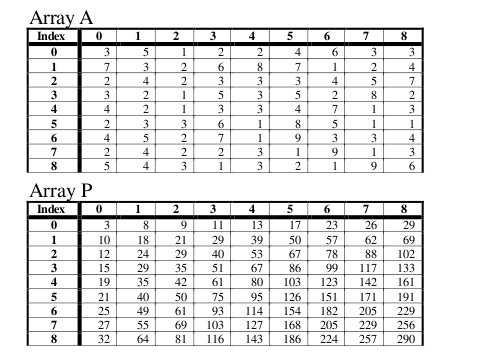
\includegraphics[scale=0.5]{prefixtable.png}
\cite{Geffner99}
\end{frame}

\begin{frame}{Updating the Prefix-Sum Table}
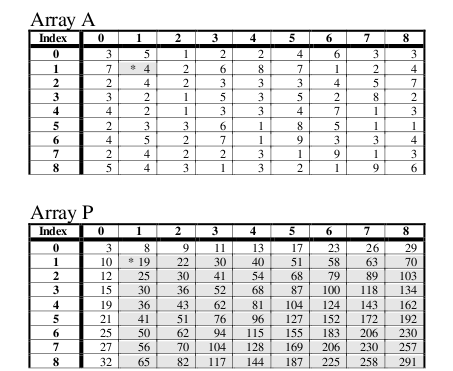
\includegraphics[scale=0.5]{prefixupdate.png}
\cite{Geffner99}
\end{frame}

\begin{frame}{Relative Prefix Method}
Geffner, Agrawal, El Abbadi, Smith\cite{Geffner99}
introduced two new tables
\begin{itemize}
    \item relative-prefix table
    \item overlay table
\end{itemize}
\end{frame}

\begin{frame}{Overlay Table - Anchor Value}
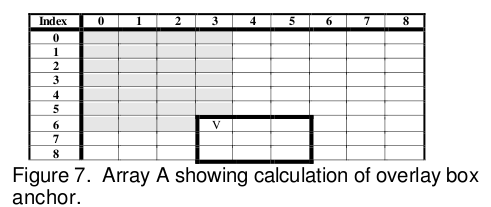
\includegraphics[scale=0.4]{relprefix_anchor.png}
\cite{Geffner99}
\end{frame}

\begin{frame}{Overlay Table - Outer Values}
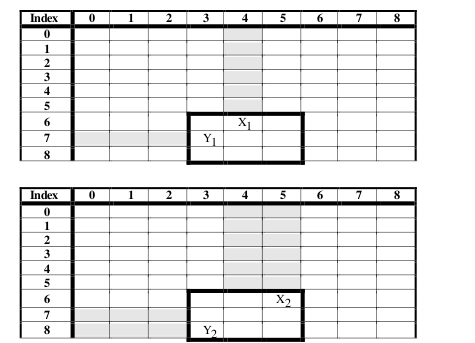
\includegraphics[scale=0.4]{relprefix_outer.png}
\cite{Geffner99}
\end{frame}

\begin{frame}{Relative Prefix Table}
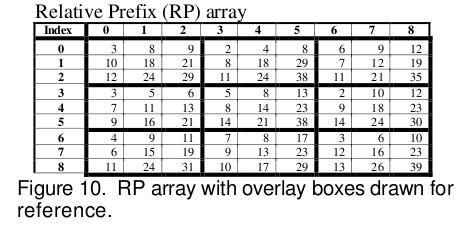
\includegraphics[scale=0.4]{relprefix_rp.png}
\cite{Geffner99}
\end{frame}

\begin{frame}{Relative Prefix Method}
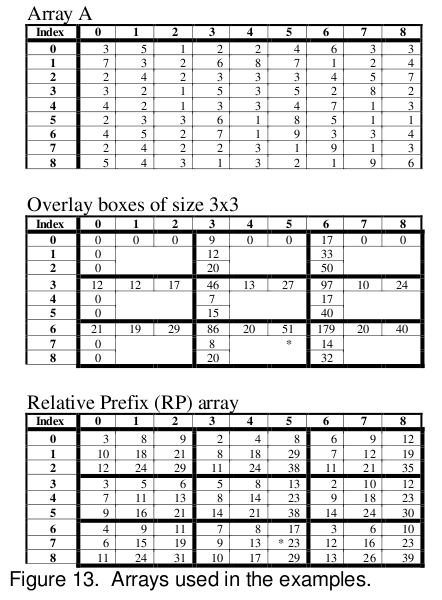
\includegraphics[scale=0.4]{relprefix_tables.png}
\cite{Geffner99}
\end{frame}

\begin{frame}{Updating Overlay and Relative Prefix Table}
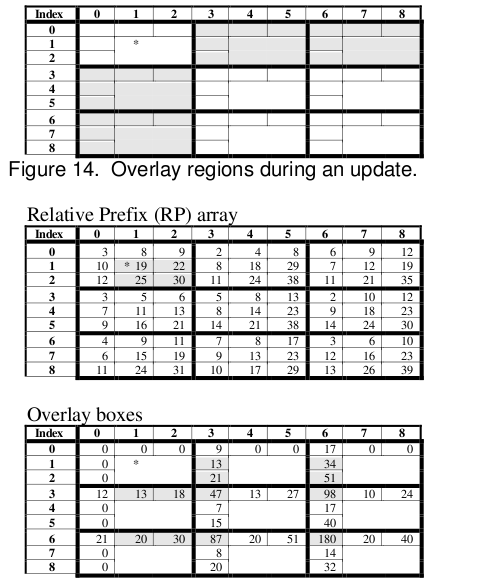
\includegraphics[scale=0.4]{relprefix_update.png}
\cite{Geffner99}
\end{frame}

\begin{frame}{Dynamic Data Cube}
\begin{figure}
    \centering
    \subfigure{
    Root:
    \begin{tabular}{ | l l l l | l l l l |}
        \hline
         Q  &  &  &  11 &  R  &  &  & 15 \\
         &  &  &  29 &  &  &  & 33 \\
         &  &  &  40 &  &  &  & 48 \\
         15 &  29 &  35 &  \textbf{51} &  16 &  35 &  \textbf{48} & 66 \\
        \hline
         S  &     &     &  10 & {\color{brown} \textbf{T}}  &    &    & 15 \\
         &   &     &  \textbf{24} &    &    &  & 31 \\
           &    &    & 42 &    &    &    & 47 \\
        12 & 26 & 34 & 52 &  8 & 30 & 54 & 61 \\
        \hline
    \end{tabular}
    }

    {\color{brown} \textbf{T}}:
    \subfigure{
    \begin{tabular}{ | l l | l l |}
        \hline
         U &  7 &  {\color{blue} \textbf{V}} & 8 \\
         4 &   \textbf{16} &  \textbf{12}{\color{red} *} & 15 \\
        \hline
        W & 10 & Z & 6 \\
        4 & 14 & 12 & 16 \\
        \hline
    \end{tabular}
    }
    {\color{blue} \textbf{V}}:
    \subfigure{
    \begin{tabular}{ | l | l |}
        \hline
        7 & 1 \\
        \hline
        5{\color{red} *} & 2 \\
        \hline
    \end{tabular}
    }
\end{figure}
\cite{Geffner00}
\end{frame}
\begin{frame}{Dynamic Data Cube}
\begin{figure}
    \centering
    \subfigure{
    Root:
    \begin{tabular}{ | l l l l | l l l l |}
        \hline
         Q  &  &  &  11 &  R  &  &  & 15 \\
         &  &  &  29 &  &  &  & 33 \\
         &  &  &  40 &  &  &  & 48 \\
         15 &  29 &  35 &  \textbf{51} &  16 &  35 &  \textbf{48} & 66 \\
        \hline
         S  &     &     &  10 & {\color{brown} \textbf{T}}  &    &    & 15 \\
         &   &     &  \textbf{24} &    &    &  {\color{red} *} & 31 \\
           &    &    & 42 &    &    &    & 47 \\
        12 & 26 & 34 & 52 &  8 & 30 & 54 & 61 \\
        \hline
    \end{tabular}
    }

    {\color{brown} \textbf{T}}:
    \subfigure{
    \begin{tabular}{ | l l | l l |}
        \hline
         U &  7 &  {\color{blue} \textbf{V}} & 8 \\
         4 &   \textbf{16} &  \textbf{12}{\color{red} *} & 15 \\
        \hline
        W & 10 & Z & 6 \\
        4 & 14 & 12 & 16 \\
        \hline
    \end{tabular}
    }
    {\color{blue} \textbf{V}}:
    \subfigure{
    \begin{tabular}{ | l | l |}
        \hline
        7 & 1 \\
        \hline
        5{\color{red} *} & 2 \\
        \hline
    \end{tabular}
    }
\end{figure}
\cite{Geffner00}
\end{frame}

\begin{frame}{Dynamic Data Cube}
\begin{figure}
    \centering
    \subfigure{
    Root:
    \begin{tabular}{ | l l l l | l l l l |}
        \hline
        \graycell Q  & \graycell & \graycell & \graycell 11 & \graycell R  & \graycell & \graycell & 15 \\
        \graycell & \graycell & \graycell & \graycell 29 & \graycell & \graycell & \graycell & 33 \\
        \graycell & \graycell & \graycell & \graycell 40 & \graycell & \graycell & \graycell & 48 \\
        \graycell 15 & \graycell 29 & \graycell 35 & \graycell \textbf{51} & \graycell 16 & \graycell 35 & \graycell \textbf{48} & 66 \\
        \hline
        \graycell S  & \graycell    & \graycell    & \graycell 10 & {\color{brown} \textbf{T}}  &    &    & 15 \\
        \graycell & \graycell  & \graycell    & \graycell \textbf{24} &    &    &  {\color{red} *} & 31 \\
           &    &    & 42 &    &    &    & 47 \\
        12 & 26 & 34 & 52 &  8 & 30 & 54 & 61 \\
        \hline
    \end{tabular}
    }

    {\color{brown} \textbf{T}}:
    \subfigure{
    \begin{tabular}{ | l l | l l |}
        \hline
        \graycell U & \graycell 7 & \graycell {\color{blue} \textbf{V}} & 8 \\
        \graycell 4 & \graycell  \textbf{16} & \graycell \textbf{12}{\color{red} *} & 15 \\
        \hline
        W & 10 & Z & 6 \\
        4 & 14 & 12 & 16 \\
        \hline
    \end{tabular}
    }
    {\color{blue} \textbf{V}}:
    \subfigure{
    \begin{tabular}{ | l | l |}
        \hline
        7 & 1 \\
        \hline
        5{\color{red} *} & 2 \\
        \hline
    \end{tabular}
    }
\end{figure}
\cite{Geffner00}
\end{frame}

%\begin{frame}{$\Delta$-tree}
%\end{frame}

\begin{frame}
\footnotesize
\bibliography{slides}{}
\bibliographystyle{plain}
\end{frame}

%\begin{frame}{The Range-Sum Problem}
%\textbf{Range queries} ``apply a given aggregation operation over selected cells where the selection is specified as contiguous ranges in the domains of some of the attributes''
%\end{frame}

\begin{frame}
\textbf{Slides} \\
\url{github.com/paulgb/cumc2010/raw/master/slides.pdf} \\
\vspace{1.5em}
\textbf{Try Sage!} \\
\url{sagemath.org}
\end{frame}

\end{document}

